% OakGPT Chat C1 report. LaTeX source of report.md; the two must stay in sync.
% Build (pdfLaTeX, XeLaTeX or Tectonic): run twice from this directory, e.g.
%   pdflatex report.tex && pdflatex report.tex
% The source is pure ASCII so every engine accepts it.
\documentclass[11pt,a4paper]{article}

\usepackage{iftex}
\ifPDFTeX
  \usepackage[T1]{fontenc}
  \usepackage{lmodern}
\fi
\usepackage[margin=25mm]{geometry}
\usepackage{microtype}
\usepackage{booktabs}
\usepackage{tabularx}
\usepackage{array}
\usepackage{graphicx}
\usepackage{xcolor}
\usepackage{enumitem}
\usepackage{fancyvrb}
\usepackage{caption}
\usepackage{float}
\usepackage[hidelinks]{hyperref}

\definecolor{oak}{HTML}{3F6B3A}
\hypersetup{colorlinks=true,linkcolor=oak,urlcolor=oak,citecolor=oak,
  pdftitle={OakGPT Chat C1: A Local Multi-Turn Assistant on Consumer Hardware},
  pdfauthor={OakGPT - Local LLM}}
\setlist{itemsep=2pt,topsep=4pt}
\setlength{\parindent}{0pt}
\setlength{\parskip}{6pt}
\newcolumntype{Y}{>{\raggedright\arraybackslash}X}
\renewcommand{\arraystretch}{1.15}
\urlstyle{same}

\newcommand{\code}[1]{\texttt{#1}}
\newcommand{\decision}[1]{\subsection*{#1}\addcontentsline{toc}{subsection}{#1}}
\newcommand{\field}[1]{\textbf{#1}\quad}

\title{\textbf{OakGPT Chat C1: A Local Multi-Turn Assistant\\on Consumer Hardware}\\[4pt]
  \large Design decisions, rationale, sources and measured results}
\author{OakGPT -- Local LLM}
\date{2026-11-22}

\begin{document}
\maketitle

\begin{center}
\small
\begin{tabularx}{0.9\textwidth}{@{}lY@{}}
\toprule
Track & Chat, stage C1 (independent of the robotics phase numbering) \\
Branch & \path{feature/chat-c1-local-web-chat} \\
Implementation commit & \code{c4a290e} \\
Hardware & NVIDIA GeForce RTX 2060, 6\,GB VRAM, driver 560.94, Windows 10 19045 \\
Inference & llama.cpp \code{b11930-85cc432e2}, Qwen3 1.7B Q4\_K\_M from Phase 2 \\
\bottomrule
\end{tabularx}
\end{center}

\begin{abstract}
\noindent OakGPT C1 adds a ChatGPT-style assistant to the project that runs entirely on
one consumer PC. A browser UI streams replies from Qwen3 1.7B, which is served by a
loopback llama.cpp process. It keeps multi-turn history, supports a selectable reasoning
mode and stores conversations as local files. Nothing is sent to a remote service.

Conversation formatting matches the model's own chat template at the token level. A live
test against the GGUF template and tokenizer confirms this. Message text cannot create
role delimiters. Enabling the llama.cpp prompt cache lowers median time to first token at
the eighth turn from 215\,ms to 55\,ms in a paired study. The cost is greedy outputs that
differ from uncached evaluation.

This report records each important decision with its alternatives, justification,
evidence and sources. It also records what was not measured. C1 is a
product-engineering stage. It makes no claim about answer quality; no chat quality
evaluation was run.
\end{abstract}

\tableofcontents

% ---------------------------------------------------------------------------
\section{Goal and scope}

The goal is a portfolio-quality ``own ChatGPT'': a usable, private assistant that shows
end-to-end engineering on limited hardware. C1 covers:
\begin{itemize}
  \item the chat interaction (multi-turn history, streaming, stop and regenerate, system
        prompt, reasoning mode)
  \item local persistence
  \item a browser UI
  \item security appropriate to a local web service
  \item reproducible latency and memory measurements
\end{itemize}
C1 explicitly excludes fine-tuning. That is planned as stage C2, a separately measured
hypothesis (Section~\ref{sec:next}).

% ---------------------------------------------------------------------------
\section{System overview}

\begin{Verbatim}[fontsize=\small,frame=single,framesep=3mm]
Browser (index.html + app.js, same origin only)
   |  fetch + Server-Sent Events, JSON only
   v
oakgpt chat  (Python standard library, 127.0.0.1:8765)
   |-- server.py    Host/Origin/Fetch-Metadata checks, CSP, routing, SSE
   |-- store.py     one JSON file per conversation, atomic replace (runs/chat/)
   |-- engine.py    context planning, sampling presets, stream statistics
   |-- template.py  Qwen3 ChatML rendering as (text, control) segments
   `-- reasoning.py incremental <think> / answer separation
   |  native token IDs, loopback HTTP, proxies bypassed
   v
llama-server b11930 (127.0.0.1:18080, --parallel 1, -c 8192, -ngl 99)
   `-- phase2-Qwen3-1.7B-Q4_K_M.gguf on the RTX 2060
\end{Verbatim}

The command
\begin{center}\code{oakgpt chat --config configs/chat/qwen3\_q4km.json}\end{center}
starts and supervises llama-server. It verifies that the server loaded the configured model path, then opens
the UI. \code{oakgpt chat-measure} runs the latency study in Section~\ref{sec:results}.

% ---------------------------------------------------------------------------
\section{Decision records}

Each record states the decision, the alternatives considered, the justification and its
consequences. Bracketed numbers refer to the references at the end.

\decision{D1. Build the assistant on a pretrained model, not the scratch Transformer}

\field{Decision.} Serve Qwen3 1.7B, a pretrained instruction-tuned model, as the
assistant. The OakGPT scratch Transformer remains a research artifact.

\field{Alternatives.} Instruction-tune the scratch model for chat, or offer both.

\field{Justification.} The best Phase 2 scratch model reaches a test NLL of 2.8459 per
byte token on WikiText~\cite{phase2}. Phase 2 calls this ``an early-budget engineering
baseline, not a converged architecture ranking''. A model of that size and training
budget cannot hold a useful conversation. Qwen3 1.7B is trained by its authors for both a
thinking and a non-thinking chat mode~\cite{qwencard,qwenreport}. It already runs locally
at about 87 decoded tokens/s on this GPU~\cite{phase2}. The portfolio value of C1 lies in
the system around the model. Training remains a separate, honestly evaluated track (C2).

\field{Consequences.} The UI states that a small local model makes mistakes. Model
licensing follows the upstream Apache 2.0 declaration recorded in the README.

\decision{D2. Separate chat track and branch}

\field{Decision.} Name the work ``Chat C1'' and branch from the current HEAD of
\path{remediation/phase33-executor-restart}, not from \code{main}.

\field{Justification.} ``Phase 4'' already means the robotics gate, which the Phase 3.3
evaluation recorded as \textbf{NO-GO}. Reusing the label would make that record
ambiguous. Branching from the current HEAD keeps README and roadmap edits free of
conflicts with the 13 unmerged robotics commits. The user chose this. The chat package
does not depend on robotics code.

\decision{D3. Default quantization: Q4\_K\_M, with Q8\_0 as an alternative configuration}

\field{Decision.} \path{configs/chat/qwen3_q4km.json} is the default.
\path{configs/chat/qwen3_q8.json} is kept as an alternative.

\field{Evidence.} The matched Phase 2 study converts both files from the same F16 GGUF,
which came from upstream revision \code{70d244cc\ldots}~\cite{phase2}. It measured:

\begin{center}
\small
\begin{tabular}{@{}lrr@{}}
\toprule
Metric (Phase 2, same hardware) & Q4\_K\_M & Q8\_0 \\
\midrule
Short-task exact accuracy, 48 prompts & 0.271 & 0.271 \\
Paired difference, bootstrap 95\% CI & \multicolumn{2}{c}{0.000 [0.000, 0.000]} \\
Median decode rate, short workload & 86.8 tok/s & 64.3 tok/s \\
Median decode rate, long workload & 93.9 tok/s & 66.4 tok/s \\
File size & 1.28 GB & 2.17 GB \\
\bottomrule
\end{tabular}
\end{center}

\field{Justification.} Q4\_K\_M decodes about 35\% faster and leaves more VRAM for the
KV cache (D4). Phase 2 observed no accuracy difference.

\field{Limitation.} That accuracy comparison uses one narrow, strictly scored task. ``No
observed difference'' does not establish equivalence for open-ended chat. This is why the
Q8\_0 configuration is kept.

\field{Provenance correction.} The first draft of the configuration copied the model
revision of the official Q8 GGUF repository. The Phase 2 files descend from a different
upstream revision (\code{70d244cc86ccca08cf5af4e1e306ecf908b1ad5e}). This was caught and
corrected before commit. The configuration now points to
\path{reports/phase2/quantization_artifacts.json}.

\decision{D4. Context length: 8192 tokens}

\field{Decision.} Start llama-server with \code{-c 8192}.

\field{Calculation.} The GGUF metadata gives 28 layers, 8 KV heads and a key/value length
of 128. An f16 KV cache therefore needs
$2 \times 28 \times 8 \times 128 \times 2\,\mathrm{B} = 112\,\mathrm{KiB}$ per token.
That is 896\,MiB at 8192 tokens and 3.5\,GiB at the model's full 40960-token context. The
full context does not fit next to the 1.2\,GiB model and the desktop's own usage of about
1.4\,GiB.

\field{Measurement.} With the server loaded and idle, device-wide memory use rose from
1418--1423\,MiB to 3530--3534\,MiB, an increase of about 2110\,MiB
(\path{vram_v1.txt}). These \code{nvidia-smi} samples cover the whole device, not just
the server process. They were taken at idle, so the peak during generation was not
measured. About 2.6\,GiB stayed free in that state.

\field{Consequences.} Long conversations are windowed (D8). Q8\_0 at 8192 tokens was not
measured. The estimate is about 0.9\,GiB more for the larger model file.

\decision{D5. Keep llama.cpp's native API with an explicit client-side template}

\field{Decision.} OakGPT renders the Qwen3 ChatML itself and sends the prompt to the
native \code{/completion} endpoint as a token-ID array. It does not use the
OpenAI-compatible \path{/v1/chat/completions} endpoint.

\field{Alternatives.} Use the OpenAI-compatible endpoint with the server-side Jinja
template, or use an external chat framework.

\field{Justification.}
\begin{itemize}
  \item The existing, tested Phase 1 client already uses the native API, with
        loopback-only URLs, proxy bypass and native token counts.
  \item Rendering client-side makes the template inspectable and testable on CPU.
  \item Only client-side rendering allows the token-level role boundary in D6.
  \item llama.cpp documents that array prompts are evaluated as given. A BOS token is
        only inserted when the prompt is a string or starts with one~\cite{llamacpp}.
\end{itemize}

\field{Verification.} \path{test_chat_template_and_tokens_match_live_gguf_template} asks
the live server's \code{/apply-template}, which runs the template embedded in the GGUF.
It runs with thinking on and off, over a conversation that includes reasoning, Markdown
and a system prompt. The rendered text matched exactly. The token IDs also matched the
server's tokenization of the whole rendered string. A recorded copy of that output is the
CPU golden test.

\decision{D6. Message content can never become control tokens}

\field{Decision.} Template delimiters are tokenized with \code{parse\_special=true}.
Message content is tokenized with \code{parse\_special=false}.

\field{Evidence.} On the pinned server, tokenizing the text \verb+<|im_end|>hi+ gives
\code{[151645, 6023]} with special parsing: one control token. Without special parsing it
gives \code{[27, 91, 318, 6213, 91, 29, 6023]}: ordinary text. Without D6, pasting text
that contains ChatML markers would forge a turn boundary. That could be a log file, or an
excerpt from this report. Unit tests check that no message content enters a control
segment. A server test checks that hostile content reaches the model as plain-text token
IDs.

\field{Scope.} OWASP lists ``Segregate and identify external content'' as a mitigation
for prompt injection~\cite{owaspllm}. D6 implements that separation at the token level.
It does \textbf{not} stop the model from following instructions written in plain
language; OWASP notes it is ``unclear if there are fool-proof methods of
prevention''~\cite{owaspllm}. With one local user and no tools, a successful injection
can only produce text.

\decision{D7. Two modes with model-card sampling; reasoning removed from history}

\field{Decision.} The UI offers \textbf{Fast}, which is non-thinking, and
\textbf{Reasoning}, which is thinking. The presets use exactly the model card's
recommendations~\cite{qwencard}:

\begin{center}
\small
\begin{tabular}{@{}llrrrrr@{}}
\toprule
Preset & Thinking & Temperature & TopP & TopK & MinP & Reply limit \\
\midrule
\code{chat} (Fast) & off & 0.7 & 0.8 & 20 & 0 & 1024 tokens \\
\code{reasoning} & on & 0.6 & 0.95 & 20 & 0 & 4096 tokens \\
\bottomrule
\end{tabular}
\end{center}

\field{Justification.} The model card says ``DO NOT use greedy decoding'' in thinking
mode. For multi-turn use it also says ``the historical model output should only include
the final output part and does not need to include the thinking content''~\cite{qwencard}.
The renderer follows that rule, using the same split rule as the GGUF template. The
reasoning text is still stored and shown in a collapsible ``Thought process'' block.
\code{presence\_penalty} defaults to 0, because the card warns that higher values ``may
occasionally result in language mixing''~\cite{qwencard}. It can be set per request; the
card suggests 1.5 only if endless repetition occurs.

\field{Implementation note.} Stream chunks can split \verb+<think>+, \verb+</think>+ and
the newlines around them. Tests found two real bugs where a newline leaked into the
reasoning text when a chunk boundary fell next to a tag. Both were fixed. Every chunk
size from 1 to 100 characters now yields identical output.

\decision{D8. Context overflow: drop the oldest whole exchanges, visibly}

\field{Decision.} When the prompt plus the reply budget would exceed the context, the
engine leaves out the oldest complete user/assistant exchanges, one at a time. The system
prompt and the newest user message always stay. The UI shows how many exchanges were left
out. If the newest message alone cannot fit, the request is refused, and the user message
is rolled back so the conversation stays valid.

\field{Alternatives.}
\begin{itemize}
  \item llama.cpp's context shifting is silent and outside the client's control. The
        Phase 1 client explicitly rejects truncation.
  \item Summarizing old turns adds a model call, latency and a second opportunity for
        errors.
  \item Refusing outright forces the user to start over.
\end{itemize}

\field{Justification.} Dropping whole exchanges keeps every remaining turn well formed
and the policy is simple to state. The stored conversation is never modified.

\decision{D9. Prompt cache enabled for chat, still disabled for benchmarks}

\field{Decision.} Chat requests send \code{cache\_prompt: true}. The existing benchmark
backend is unchanged and keeps it \code{false}.

\field{Evidence.} The paired study is described in Section~\ref{sec:results}. Without
the cache, every turn re-evaluates the whole history. TTFT grows from 42\,ms to 215\,ms
over eight turns. With the cache it stays between 37 and 55\,ms.

\field{Trade-off.} llama.cpp documents that with prompt caching the logits ``are
\textbf{not} guaranteed to be bit-for-bit identical for different batch sizes'', which
``can cause nondeterministic results''~\cite{llamacpp}. This was observed. Greedy replies
were identical across all five repetitions within each condition. They differed between
conditions from the third reply onward, with the wording diverging slightly. For
interactive chat with sampling this does not matter. Measurement code therefore keeps the
cache off, and the existing quantization and benchmark records are untouched.

\decision{D10. Standard-library server, Server-Sent Events and plain JavaScript}

\field{Decision.} The web server is \code{http.server.ThreadingHTTPServer}. Streaming
uses Server-Sent Events~\cite{sse}. The UI is about 870 lines of hand-written HTML, CSS
and JavaScript with no build step. It loads no external fonts, libraries or analytics.

\field{Alternatives.} FastAPI or Flask with a SPA framework, a Gradio UI, or an existing
product such as a third-party chat frontend.

\field{Justification.}
\begin{itemize}
  \item \path{AGENTS.md} asks for small explicit implementations and standard-library
        dependencies.
  \item An existing chat frontend would hide the engineering that this portfolio stage is
        meant to show.
  \item SSE fits one-way token streaming. It needs no WebSocket upgrade and works with
        \code{fetch} plus \code{AbortController}, so pressing Stop closes the stream.
\end{itemize}

\field{Risk accepted.} Python documents that ``\code{http.server} is not recommended for
production. It only implements basic security checks''~\cite{pyhttp}. The service is
therefore restricted to loopback and one user. The checks it lacks are added explicitly
(D11).

\decision{D11. Security model for a localhost web service}

\field{Threat.} Binding to 127.0.0.1 keeps other machines out. It does not stop a
malicious website open in the same browser. Such a site can send requests to localhost,
which is cross-site request forgery. Through DNS rebinding it can also make its own
hostname resolve to 127.0.0.1 and then read responses~\cite{rebinding}.

\field{Controls and the source behind each.}

\begin{center}
\small
\begin{tabularx}{\textwidth}{@{}YYY@{}}
\toprule
Control & Defends against & Source \\
\midrule
Bind only to \code{127.0.0.1}/\code{::1}; refuse anything else at startup
  & Network access & -- \\
Exact \code{Host} allowlist (\code{127.0.0.1:<port>}, \code{localhost:<port>}),
  otherwise 421 & DNS rebinding & \cite{rebinding} \\
Reject a present \code{Origin} that is not our own
  & CSRF & OWASP, ``Using Standard Headers to Verify Origin''~\cite{owaspcsrf} \\
Reject state-changing requests with \code{Sec-Fetch-Site} other than same-origin/none
  & CSRF & OWASP, ``Fetch Metadata headers''~\cite{owaspcsrf} \\
State-changing requests must be \code{application/json}; CORS preflight always refused
  & CSRF via simple requests & OWASP, ``Disallowing simple requests''~\cite{owaspcsrf} \\
CSP \code{default-src 'self'}, \code{frame-ancestors 'none'}, \code{nosniff},
  \code{no-referrer} & Script injection, clickjacking & \cite{mdncsp} \\
Markdown renderer escapes all text before adding its own tags; links render as text
  & XSS from model output & \cite{mdncsp} \\
Strict 32-hex conversation IDs; static files from an allowlist
  & Path traversal & -- \\
256\,KiB body limit, 32,000-character messages, one generation at a time
  & Resource exhaustion & -- \\
\bottomrule
\end{tabularx}
\end{center}

OWASP makes a fallback from Fetch Metadata to origin verification
mandatory~\cite{owaspcsrf}; both are implemented. Every row except ``bind'' has a CPU test
in \path{tests/test_chat_server.py}.

\field{Not covered.} Malware already running as the same user can read the files and the
port. That is outside this threat model.

\decision{D12. Conversation storage: one JSON file per conversation}

\field{Decision.} Each conversation is stored at
\path{runs/chat/conversations/<uuid>.json} with a format tag (\code{oakgpt-chat-v1}).
Writes go to a temporary file, are flushed and \code{fsync}ed, then moved into place with
\code{os.replace}, which is atomic~\cite{pyos}.

\field{Alternatives.} SQLite from the standard library, or one combined file.

\field{Justification.} Files are human-readable, easy to delete and need no migrations. A
crash cannot corrupt an existing conversation. \path{runs/} is git-ignored, so private
conversations can never be committed, which follows the rule in \path{AGENTS.md}.

\field{Revisit.} Full-text search across many conversations would favour SQLite.

\decision{D13. One generation at a time}

\field{Decision.} llama-server runs with \code{--parallel 1}. The chat server holds a lock
and answers a second concurrent request with 409.

\field{Justification.} There is one user and 6\,GB of VRAM. llama.cpp splits the context
between parallel slots, so two slots would halve each conversation's context. Queuing
silently behind a hidden request would make the UI appear frozen.

\decision{D14. Stop semantics and partial replies}

\field{Decision.} Pressing Stop aborts the browser \code{fetch}. The next server write
then fails, which closes the upstream llama.cpp stream and stops decoding. The partial
reply is saved with \code{"interrupted": true}, so the conversation stays well formed and
the next message works immediately.

\field{Investigation.} An early end-to-end run suggested the server missed the
disconnect. It turned out the test client never released its socket: \code{http.client}
keeps the socket open through the response object. Socket probing was added, then
removed again, because a regression test showed disconnects are detected without it. Only
code with demonstrated value was kept.

\decision{D15. Provenance of every reply}

\field{Decision.} Each stored reply records:
\begin{itemize}
  \item its sampling settings, including the seed actually used (drawn per reply when not
        given)
  \item prompt token count and dropped exchanges
  \item server-reported prompt, cache and decode timings, passed through unchanged
  \item the stop reason (\code{eos} or \code{limit})
\end{itemize}
The status endpoint reports the model file, its SHA-256 (computed at startup), the server
build and the launch command. Values the server does not report are stored as
\code{null}, never estimated.

% ---------------------------------------------------------------------------
\section{Verification}

\begin{center}
\small
\begin{tabularx}{\textwidth}{@{}>{\raggedright\arraybackslash}p{0.4\textwidth}Y@{}}
\toprule
Check & Result \\
\midrule
\code{pytest} (CPU, no models) & 183 passed, 3 skipped (hardware tests skip without
  opt-in) \\
Live template parity test (hardware) & passed against llama.cpp b11930 + Q4\_K\_M \\
\code{ruff check .}, \code{ruff format --check .}, \code{mypy} (strict) & clean \\
Wheel contents & \path|oakgpt/chat/static/{index.html,app.js,style.css}| included \\
End-to-end, real model & multi-turn replies, reasoning separation, cache reuse, Stop
  then continue \\
UI, headless Edge & desktop 1280\,px and narrow 600\,px rendered correctly
  (Figures~\ref{fig:conversation}--\ref{fig:narrow}) \\
\bottomrule
\end{tabularx}
\end{center}

The narrow layout was checked only down to 600\,px. A 420\,px capture appeared clipped at
about 500\,px, which suggests a minimum window width in headless mode; phone widths below
that are unverified. The UI JavaScript has no automated browser tests.

\begin{figure}[H]
  \centering
  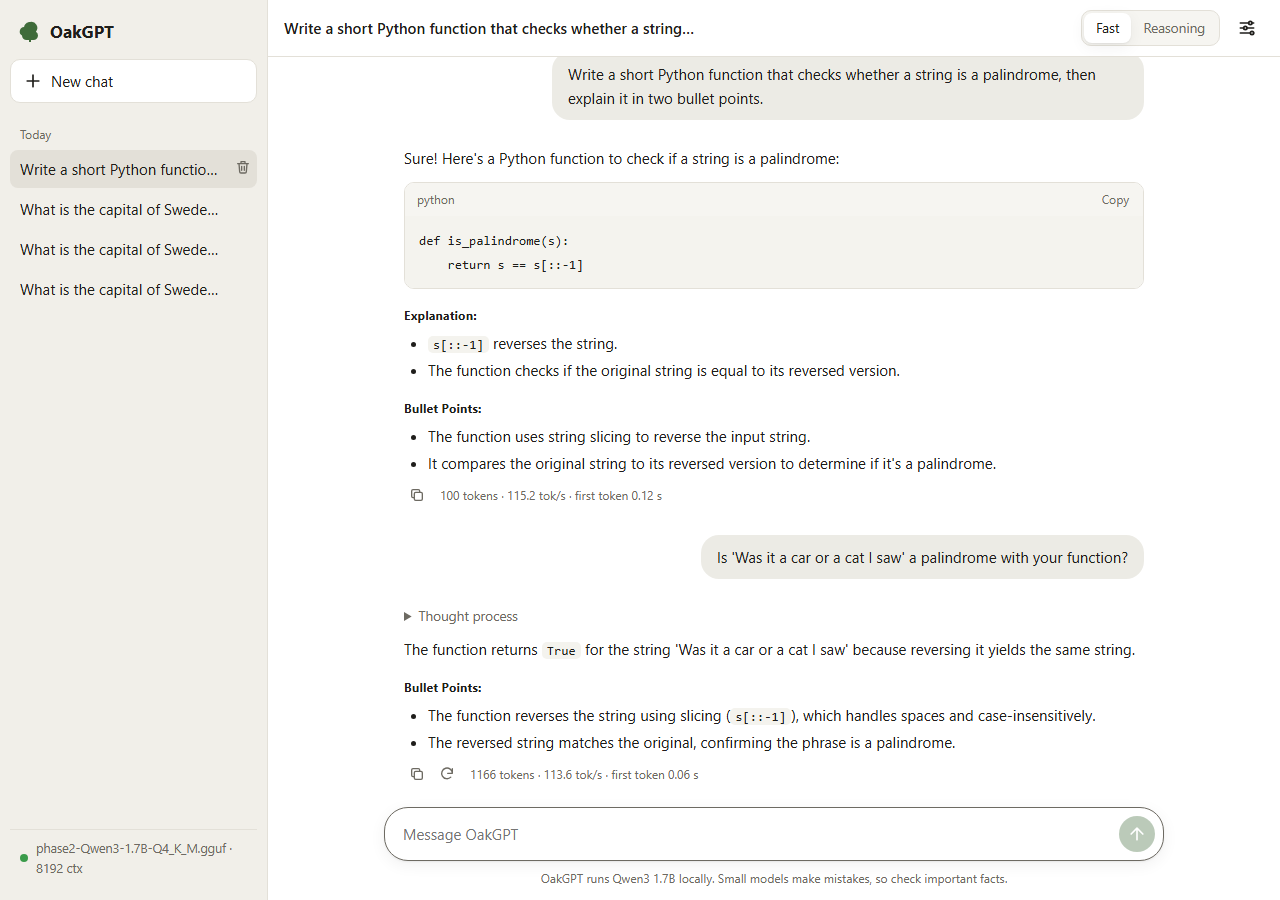
\includegraphics[width=\textwidth]{figures/ui-conversation-1280.png}
  \caption{Conversation view at 1280\,px, with a reasoning reply and per-reply
    statistics. The model's claim about the palindrome check is wrong
    (Section~\ref{sec:observed}).}
  \label{fig:conversation}
\end{figure}

\begin{figure}[H]
  \centering
  \begin{minipage}[b]{0.62\textwidth}
    \centering
    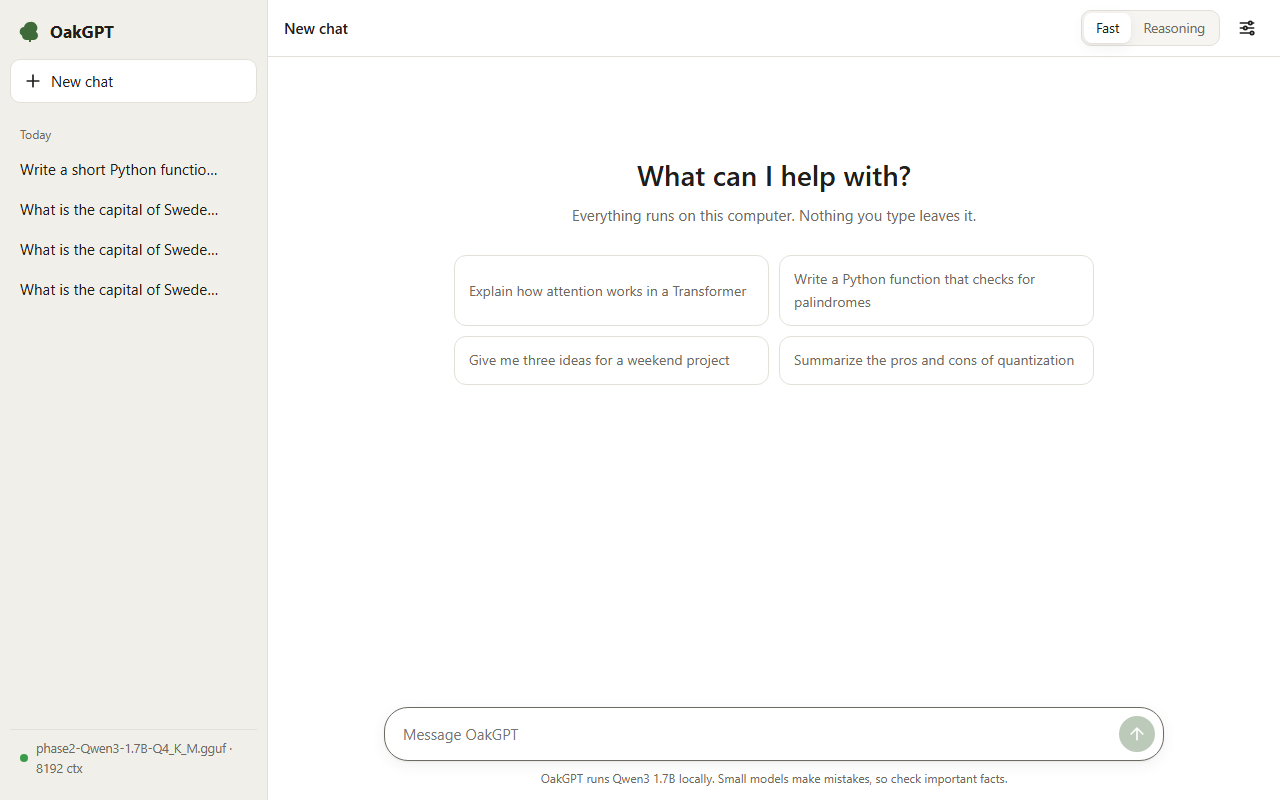
\includegraphics[width=\linewidth]{figures/ui-empty-1280.png}
    \caption{Empty state with suggestions, 1280\,px.}
    \label{fig:empty}
  \end{minipage}\hfill
  \begin{minipage}[b]{0.34\textwidth}
    \centering
    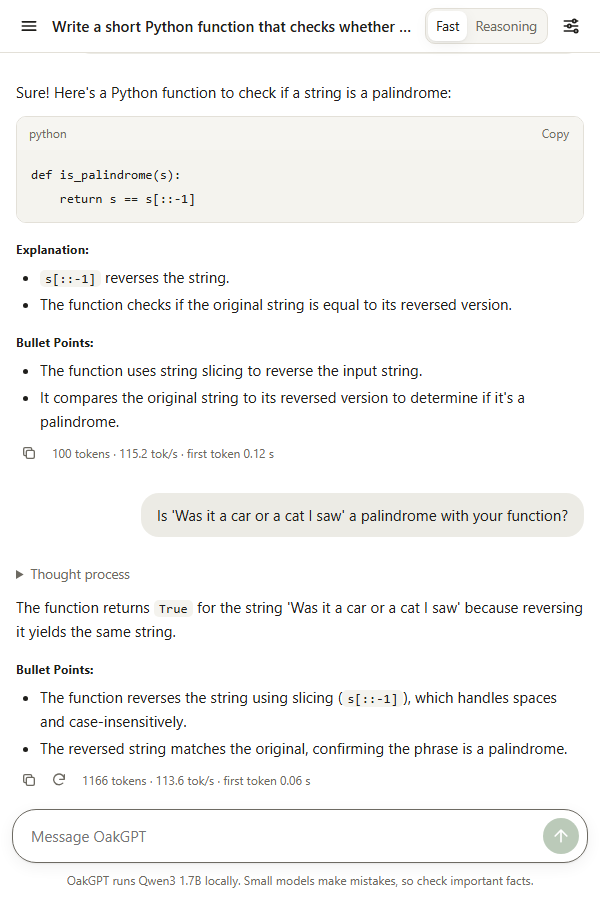
\includegraphics[width=\linewidth]{figures/ui-narrow-600.png}
    \caption{Narrow layout, 600\,px.}
    \label{fig:narrow}
  \end{minipage}
\end{figure}

% ---------------------------------------------------------------------------
\section{Measured results}\label{sec:results}

\subsection{Prompt cache study (\code{cache\_study\_v1.json})}

\field{Design.}
\begin{itemize}
  \item \textbf{Script:} an original eight-turn script,
        \path{data/eval/chat_cache_script_v1.json}, which is for latency measurement only
        and is never used for training.
  \item \textbf{Decoding:} greedy, non-thinking, at most 96 new tokens per reply, seed
        2026.
  \item \textbf{Conditions:} five conversations per condition, in ABBA order on one
        server process.
  \item \textbf{Cache isolation:} before every conversation the slot cache is overwritten
        with an unrelated flush prompt, so no condition inherits the previous prefix.
  \item \textbf{Recording:} git revision \code{c4a290e}, with the working tree marked
        dirty only by untracked PDFs that predate this work. The model and binary SHA-256
        are in the raw file.
\end{itemize}

\begin{table}[H]
\centering
\small
\caption{Prompt cache on versus off, per turn. Medians over five conversations per
  condition.}
\label{tab:cache}
\begin{tabular}{@{}rrrrrr@{}}
\toprule
Turn & Prompt & Cached tokens & Server prompt ms & Median TTFT ms & Off $\div$ on \\
     & tokens & (on)          & on / off         & on / off       &  \\
\midrule
1 & 75 & 0 & 32.2 / 31.7 & 41 / 42 & 1.03 \\
2 & 150 & 71 & 31.9 / 51.5 & 37 / 56 & 1.53 \\
3 & 229 & 146 & 36.1 / 75.2 & 41 / 81 & 2.00 \\
4 & 293 & 225 & 32.4 / 95.6 & 37 / 100 & 2.73 \\
5 & 364* & 289 & 32.5 / 112.6 & 37 / 117 & 3.17 \\
6 & 459* & 353 & 42.6 / 142.5 & 47 / 147 & 3.14 \\
7 & 554* & 461 & 41.7 / 167.5 & 48 / 172 & 3.57 \\
8 & 675* & 560 & 49.6 / 209.9 & 55 / 215 & 3.94 \\
\bottomrule
\end{tabular}

\begin{minipage}{0.92\textwidth}
{\small * Prompt tokens are those of the cache-off condition. From the third reply onward
the greedy replies differ between conditions (D9), so later prompts differ by up to 10
tokens. At turn 8 the per-conversation TTFT ranged over 53--57\,ms with the cache and
209--221\,ms without. Decode rate was unaffected: 107--116 tok/s in both conditions.\par}
\end{minipage}
\end{table}



\field{Interpretation.} Without the cache, TTFT grows about linearly with history length.
With it, only the new suffix is evaluated. At these lengths the difference is tens to
hundreds of milliseconds. Near the 8192-token limit it would be larger, but that was not
measured.

\subsection{Memory}

The server loaded and idle adds about 2110\,MiB, measured device-wide (D4).

\subsection{Observed behaviour (single samples, not a benchmark)}\label{sec:observed}

In the end-to-end smoke test, a follow-up question reused 59 cached tokens and reached
its first token in 32\,ms. The first message took 154\,ms, with nothing cached.

The demonstration conversation in Figure~\ref{fig:conversation} shows a factual error.
Qwen3 1.7B says its own \verb+s == s[::-1]+ function returns \code{True} for ``Was it a
car or a cat I saw'', which ignores spaces and capital letters. This is a single
observation, kept as an honest example of the model's limits, not as a measured error
rate.

% ---------------------------------------------------------------------------
\section{Limitations and threats to validity}

\begin{itemize}
  \item \textbf{Quality.} C1 has no chat-quality evaluation. The one quality number cited
        (D3) comes from a narrow Phase 2 task.
  \item \textbf{Latency.} One host, one script, five conversations per condition and one
        model file. TTFT includes loopback HTTP and Python overhead. Other GPU users (the
        desktop) were not controlled.
  \item \textbf{Memory.} VRAM figures cover the whole device at idle. The peak during
        generation was not measured. Q8\_0 was not measured.
  \item \textbf{Browser.} UI behaviour below 600\,px and in browsers other than Edge was
        not tested. Accessibility was not audited.
  \item \textbf{Security.} The threat model is a single trusted local user. Prompt
        injection is mitigated only at the token level (D6).
\end{itemize}

% ---------------------------------------------------------------------------
\section{Development note}

While probing the llama.cpp API, an unquoted \verb+*+ in a \verb+curl --noproxy *+
command was expanded by the shell into repository filenames. curl then also sent the
requests to hostnames such as \code{README.md} and \code{MANIFEST.in}; \code{.md} and
\code{.in} are real top-level domains. The payloads were fixed test strings
(\verb+<|im_end|>hi+, \code{S}, \code{Hi}, \code{Hello}, \code{Again}) and token IDs. No
user prompts, datasets or weights were sent. The command was stopped, the user was
informed, and later probes used a Python client that can only reach 127.0.0.1.

% ---------------------------------------------------------------------------
\section{Next steps}\label{sec:next}

\begin{enumerate}
  \item \textbf{C2, fine-tuning as a measured hypothesis.} Build a frozen chat evaluation
        set first, disjoint from any training data. Then measure LoRA/QLoRA feasibility on
        6\,GB against the unchanged base model, following the existing roadmap rule that a
        fine-tune must not trade safety for a higher score.
  \item Conversation search, rename and export, and a SQLite backend if search requires
        it.
  \item Automated browser tests with a headless browser, an accessibility review and a
        narrow-viewport check below 500\,px.
  \item Measure peak VRAM during generation for Q4\_K\_M and Q8\_0, and TTFT near the
        context limit.
\end{enumerate}

% ---------------------------------------------------------------------------
\section{Reproduction}

\begin{Verbatim}[fontsize=\footnotesize,frame=single,framesep=3mm]
.\.venv\Scripts\python -m pip install -e ".[dev]"
.\.venv\Scripts\oakgpt chat --config configs/chat/qwen3_q4km.json
# Latency study (refuses to overwrite its output):
.\.venv\Scripts\oakgpt chat-measure --config configs/chat/qwen3_q4km.json `
    --script data/eval/chat_cache_script_v1.json `
    --output runs/chat/cache_study.json --repeats 5
# Live template parity test against a running server:
$env:OAKGPT_LLAMA_URL = "http://127.0.0.1:18080"
.\.venv\Scripts\python -m pytest -m hardware -k chat_template
\end{Verbatim}

These commands need \path{vendor/llama.cpp/llama-server.exe} and
\path{models/phase2-Qwen3-1.7B-Q4_K_M.gguf}. Both are produced by the Phase 2 scripts; see
the README.

% ---------------------------------------------------------------------------
\begin{thebibliography}{11}
\small

\bibitem{phase2} OakGPT Phase 2 research report and quantization records:
  \path{reports/phase2/report.md}, \path{reports/phase2/quantization/summary.json},
  \path{reports/phase2/quantization_artifacts.json}.

\bibitem{qwencard} Qwen Team, ``Qwen3-1.7B'' model card, sections ``Switching Between
  Thinking and Non-Thinking Mode'' and ``Best Practices.''
  \url{https://huggingface.co/Qwen/Qwen3-1.7B} (accessed 2026-11-22).

\bibitem{qwenreport} Qwen Team, ``Qwen3 Technical Report,'' arXiv:2505.09388, 2025.

\bibitem{llamacpp} ggml-org, llama.cpp HTTP server README, parameters \code{prompt} and
  \code{cache\_prompt}, at commit \code{85cc432e2c8b92925f17dfb8937742541312f1d4}.
  \url{https://github.com/ggml-org/llama.cpp/blob/85cc432e2c8b92925f17dfb8937742541312f1d4/tools/server/README.md}

\bibitem{owaspllm} OWASP Gen AI Security Project, ``LLM01:2025 Prompt Injection,''
  mitigation 6 ``Segregate and identify external content.''
  \url{https://genai.owasp.org/llmrisk/llm01-prompt-injection/}

\bibitem{sse} WHATWG, HTML Living Standard, ``Server-sent events.''
  \url{https://html.spec.whatwg.org/multipage/server-sent-events.html}

\bibitem{pyhttp} Python Software Foundation, \code{http.server} documentation, security
  warning. \url{https://docs.python.org/3/library/http.server.html}

\bibitem{rebinding} C.~Jackson, A.~Barth, A.~Bortz, W.~Shao and D.~Boneh, ``Protecting
  Browsers from DNS Rebinding Attacks,'' in \emph{Proc.\ 14th ACM Conference on Computer
  and Communications Security (CCS)}, 2007.

\bibitem{owaspcsrf} OWASP Cheat Sheet Series, ``Cross-Site Request Forgery Prevention
  Cheat Sheet,'' sections ``Fetch Metadata headers,'' ``Disallowing simple requests'' and
  ``Using Standard Headers to Verify Origin.''
  \url{https://cheatsheetseries.owasp.org/cheatsheets/Cross-Site_Request_Forgery_Prevention_Cheat_Sheet.html}

\bibitem{mdncsp} MDN Web Docs, ``Content-Security-Policy.''
  \url{https://developer.mozilla.org/en-US/docs/Web/HTTP/Headers/Content-Security-Policy}

\bibitem{pyos} Python Software Foundation, \code{os.replace} documentation.
  \url{https://docs.python.org/3/library/os.html#os.replace}

\end{thebibliography}

\end{document}
